\documentclass[english, a4paper]{article}

\usepackage[utf8]{inputenc}
\usepackage[T1]{fontenc}
\usepackage[english]{babel}
\usepackage{lmodern}
\usepackage[top=1.7cm, right=1.8cm, bottom=1.8cm, left=1.8cm, head=14pt]{geometry}
\usepackage{calc}
\usepackage{graphicx}
\usepackage{amsmath}
\usepackage{tabularx}
\usepackage{booktabs}
\usepackage[official]{eurosym}
\usepackage{lastpage}
\usepackage{subcaption}
\usepackage{etoolbox}
\usepackage{amssymb}
\usepackage{enumitem}
\usepackage{natbib}
\usepackage{siunitx}
\usepackage[hang,flushmargin]{footmisc}
\usepackage{float} % for [H] figure placement
\usepackage[export]{adjustbox}

% spacing
\usepackage{caption}
\captionsetup{font=small}

\captionsetup[figure]{skip=5pt}
\captionsetup[subfigure]{font=scriptsize, skip=1pt}
\captionsetup[table]{skip=6pt}

\setlength{\textfloatsep}{9pt plus 1pt minus 2pt}
\setlength{\floatsep}{6pt plus 1pt minus 2pt}
\setlength{\intextsep}{8pt plus 1pt minus 2pt}
\setlength{\abovecaptionskip}{3pt}
\setlength{\belowcaptionskip}{0pt}

\bibliographystyle{plainnat}

% TikZ setup
\usepackage{tikz}
\usetikzlibrary{arrows.meta, positioning, shapes, calc, fit}

% Line spacing
\usepackage{setspace}
\setstretch{1.15}

% Page header
\usepackage[automark]{scrlayer-scrpage}
\pagestyle{scrheadings}
\clearpairofpagestyles
\ihead{}
\chead{}
\ohead{\pagemark}

% Hyperref (should come last)
\usepackage[
  colorlinks=false,
  pdfborder={0 0 0}
]{hyperref}


% \setlength{\parindent}{0pt}
\usepackage{parskip}
\usepackage{wrapfig}

%-------------- Ende allgemeine Angaben -----------------------------
\begin{document}

%-------------- Beginn Titelseite -----------------------------------
\hypersetup{pageanchor=false}
\thispagestyle{empty}
\noindent \hfill 
\includegraphics[height=2.4cm, trim=1.2cm 1.2cm 1.2cm 1.2cm]{Figures/UniKonstanz_Logo_Optimum_sRGB.jpg}

\vspace{1cm}
\begin{center}


\vspace{5cm}



\vspace{2cm}
\begin{center}
  {\Huge Deep Learning Project}
\end{center}



\vspace{3cm}
Instructor: Giordano De Marzo \\
Course: Deep Learning for Social Scientists Summer Semester 2026 \\
\end{center}

\vspace{5cm}
\begin{flushleft}
{Lisanne Dolleman, Enrolment Number: 01/1594416} \\ 
{David Marasek, Enrolment No: 01/923631} \\
{Simone Mazzoli, Enrolment No: 01/1586813} \\ 
{Aaron Siebert, Enrolment No: 01/1590814} \\

{M.Sc. Social and Economic Data Science} \\

\vspace{1cm}
Handed in: \
Konstanz, 31.08.2026\
\end{flushleft}
%-------------- Ende Titelseite -------------------------------------

%------------------ Table of Contents
\newpage
\hypersetup{pageanchor=true}
\pagenumbering{Roman}
\renewcommand{\thepage}{\Roman{page}}
\tableofcontents{}


%------------------ Main Content
\newpage
\pagenumbering{arabic}
\renewcommand{\thepage}{\arabic{page}}

%------------------ Sections


\begin{abstract}

Despite the well-established consequences of air pollution for human health, accurately measuring its spatial distribution remains a challenge. High-quality monitoring stations provide reliable measurements but their spatial coverage remains uneven. In this project, we estimate annual PM$_{2.5}$ from publicly available satellite and contextual data. We compare a multimodal CNN trained from scratch with a ResNet-50 pretrained on BigEarthNet. We also investigate whether low-cost Sensor.Community measurements can be calibrated well enough to increase the number of available training labels.

The tested annual calibration approaches strongly reduce the very large error of the raw low-cost measurements but they do not produce reliable reference-equivalent annual labels. A daily calibration using HYRAS humidity and temperature shows that weather information can explain part of the short-term sensor error. This improvement does not carry over to annual calibration. We therefore use official European Environment Agency reference measurements as final labels. Under geographic cross-validation, the scratch CNN outperforms the evaluated ResNet-50 configurations. The selected scratch model improves RMSE by 14.6\% over a training-mean baseline on a sealed northern and eastern German test region but it also shows a strongly negative $R^2$ and systematic overprediction. Finally, the Kreis-level socioeconomic analysis finds only weak and inconsistent associations between modeled PM$_{2.5}$ and the selected socioeconomic indicators.

\end{abstract}


\section{Introduction}
\label{sec:introduction}

Exposure to fine particulate matter (PM$_{2.5}$) is a well-established risk factor for cardiovascular and respiratory diseases \citep{who2021airquality}. Measuring its spatial distribution is therefore important for environmental monitoring and public-health policy. High-quality reference stations are expensive to operate and remain unevenly distributed across space. Satellite observations provide much broader geographic coverage and can therefore be used as inputs for models that estimate ground-level pollution between monitoring locations \citep{scheibenreif2021airpollution}.

This project focuses on spatial generalization rather than random interpolation between nearby stations. We keep a large northern and eastern German region separate from model development and use it only for the final evaluation. The goal is to test whether a model trained on reference stations elsewhere in Europe can transfer to a geographically distinct German region with comparatively sparse monitoring coverage.

We compare two main CNN approaches. The first is a multimodal CNN trained from scratch. The second uses a ResNet-50 pretrained on BigEarthNet for the high-resolution Sentinel-2 branch. Both models combine local and wider-context Sentinel-2 imagery with Sentinel-5P atmospheric information and elevation data. We also test different ResNet training strategies including a frozen pretrained backbone and a fully trainable variant.

A second part of the project investigates whether the much denser Sensor.Community network can supplement the official reference measurements. Low-cost particulate-matter sensors are attractive because of their spatial coverage but their measurements can be affected by device-specific errors and environmental conditions such as humidity \citep{benabbas2019particulate,weissert2023moma}. We therefore test several calibration approaches before deciding whether these measurements are suitable as annual model labels.

Finally, we apply the selected model to a regular prediction grid in the held-out German region and aggregate the resulting estimates to Kreis level. We then examine whether modeled ambient PM$_{2.5}$ is associated with selected socioeconomic and demographic indicators. This final analysis is exploratory because the pollution values are model predictions rather than direct measurements and the Kreis-level measure is not population-weighted.


\subsection{Pipeline Overview}
\label{sec:pipeline}

Figure~\ref{fig:pipeline_overview} summarizes the project pipeline. We first collect low-cost sensor measurements, official reference measurements, remote-sensing inputs and socioeconomic data. The Sensor.Community measurements are evaluated against official reference stations before model training. Since the tested annual calibration approaches are not sufficiently reliable, only EEA reference measurements are used as final training labels.

The reference measurements are co-located with the satellite and contextual inputs. These paired observations are then used to train the scratch CNN and the pretrained ResNet variants under the same geographic validation design. After model selection, the chosen scratch model is trained on the available development data and evaluated once on the sealed German test region. It is then applied to a dense prediction grid. The grid predictions are combined with Kreis-level socioeconomic data for the final exploratory analysis.

\begin{figure}[ht]
    \centering
    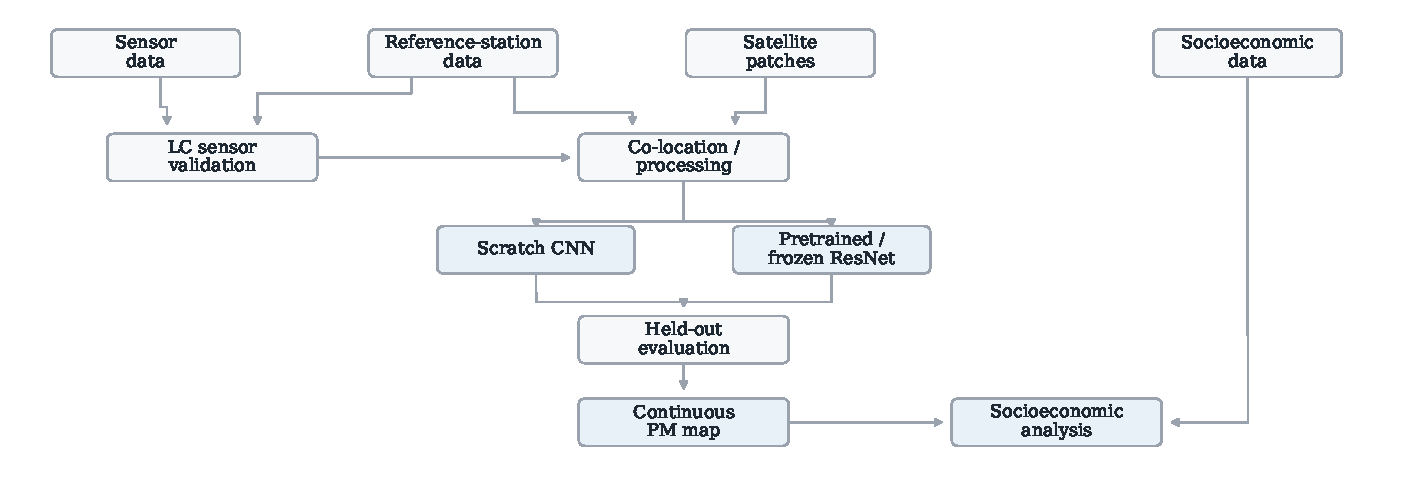
\includegraphics[width=0.9\textwidth]{Figures/generated/pipeline_overview_compact.pdf}
    \caption{Pipeline Overview.}
    \label{fig:pipeline_overview}
\end{figure}

The remainder of this report is structured as follows. Section~\ref{sec:data} describes the data and preprocessing. Section~\ref{sec:calibration} summarizes the Sensor.Community calibration experiments. Section~\ref{sec:models} describes the models and training design. Section~\ref{sec:results} presents the predictive results. Section~\ref{sec:socioeconomic} presents the socioeconomic analysis and Section~\ref{sec:conclusion} concludes.


\section{Data Collection and Processing}
\label{sec:data}

We use three main categories of data: ground-level particulate-matter measurements, remote-sensing inputs and socioeconomic data. Unless stated otherwise, the pollution and remote-sensing data refer to 2024.


\subsection{PM Data}
\label{sec:pm_data}

We initially consider two sources of ground-level particulate-matter measurements. Low-cost measurements are obtained from Sensor.Community while official reference measurements are obtained through the European Environment Agency (EEA). The Sensor.Community network provides much denser spatial coverage. The EEA network provides the higher-quality measurements needed for calibration and final model evaluation.

For the EEA data, invalid or flagged observations, missing values and negative concentrations are removed before aggregation. Remaining observations are first averaged at station-day level and then aggregated to annual station means. A 90\% station-level completeness criterion is applied during annual preprocessing. For the PM$_{2.5}$ modeling task, the model loader subsequently keeps only stations with a valid PM$_{2.5}$ target and all required remote-sensing inputs. Annual values above \SI{120}{\micro\gram\per\cubic\meter} for PM$_{10}$ and \SI{80}{\micro\gram\per\cubic\meter} for PM$_{2.5}$ are excluded as extreme values.

% TODO before submission: verify PM2.5-specific completeness among final model-ready stations.
% The cleaning script applies the 90% criterion during joint PM10/PM2.5 preprocessing.

The target transformation is applied inside the model-training pipeline rather than during initial data construction. Annual PM$_{2.5}$ is log-transformed and standardized using statistics computed from the corresponding training data. Predictions are transformed back to the original concentration scale for evaluation.

Figure~\ref{fig:coverage_validation} shows the model-ready reference-station coverage and geographic validation design. The development set contains 1,869 stations. A separate northern and eastern German test region contains 164 stations and is not used during model selection. We use a larger contiguous region instead of a single Land to create a more demanding spatial-generalization test while still retaining enough reference stations for evaluation.

\begin{figure}[ht]
    \centering
    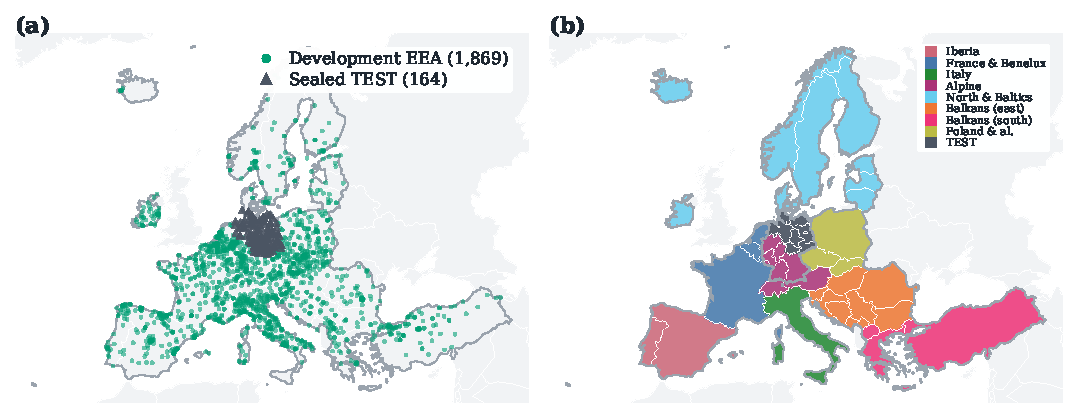
\includegraphics[width=\textwidth]{Figures/generated/coverage_validation_geography.pdf}
    \caption{Reference-station coverage and geographic validation design. Panel (a) shows the development and sealed TEST stations. Panel (b) shows the eight geographic development folds and the held-out German test region.}
    \label{fig:coverage_validation}
\end{figure}


\subsection{Satellite Data}
\label{sec:satellite}

Satellite data are extracted through Google Earth Engine (GEE). For each reference-station location, we create two Sentinel-2 surface-reflectance inputs. The high-resolution patch contains $120\times120$ pixels at \SI{10}{\meter} per pixel which corresponds to approximately $1.2\times1.2$ km. The low-resolution patch contains $60\times60$ pixels at \SI{200}{\meter} per pixel and covers approximately $12\times12$ km.

Sentinel-2 scenes with more than 20\% reported cloud coverage are excluded before an annual median composite is constructed. We retain ten bands: B2, B3, B4, B5, B6, B7, B8, B8A, B11 and B12. This band selection is compatible with the BigEarthNet-pretrained ResNet-50 used in the transfer-learning comparison.

During training, the Sentinel-2 inputs are augmented using rotations and flips. The selected evaluation pipeline uses eight test-time augmentation views. This averages predictions across equivalent image orientations and reduces sensitivity to the arbitrary orientation of a patch.


\subsection{Pollution Covariates}
\label{sec:covariates}

In addition to Sentinel-2 imagery, the model receives broader atmospheric and topographic context. Tropospheric NO$_2$ and CO from Sentinel-5P are extracted as $5\times5$ annual-mean patches at approximately \SI{7}{\kilo\meter} per pixel. A wider absorbing-aerosol-index input uses $31\times31$ pixels at the same approximate resolution which corresponds to a context of about 217 km across.

Elevation is obtained from the Copernicus GLO-30 digital elevation model. It is represented as a $60\times60$ patch resampled to \SI{200}{\meter} per pixel. The different spatial scales are intended to represent both the local land-surface environment and wider atmospheric conditions that may affect ground-level PM$_{2.5}$.


\subsection{Socio-Economic Data}
\label{sec:socio_data}

The socioeconomic dataset covers all 400 German Kreise and combines several official sources. Population, age structure, median age and population density are taken from Eurostat and refer to 2024 \citep{eurostat_pjanaggr3,eurostat_pjanind3,eurostat_d3dens}. Kreis-level unemployment rates for 2024 are obtained from the Federal Employment Agency \citep{ba_arbeitslosenquoten2024}. Disposable household income per capita refers to 2023 and comes from the Regional Accounts of the German States \citep{vgrdl_r2b3_2023}. Immigration-history and educational-attainment indicators are based on the 2022 German Census \citep{zensus2022_demografie,zensus2022_bildung}. Administrative identifiers and Kreis boundaries are based on BKG geodata \citep{bkg_vg250_2024}.

The different reference years reflect the most recent Kreis-level data available from the respective sources. We therefore treat the variables as broadly contemporaneous rather than as measurements from one identical year. Immigration history is used as a demographic characteristic rather than as a direct indicator of socioeconomic disadvantage. Population density is treated as a structural measure of urbanicity that may be related to both socioeconomic conditions and pollution.


\section{Calibration of LC PM Sensors}
\label{sec:calibration}

Sensor.Community initially looked attractive because it provides many more measurement locations than the official network. We therefore tested whether the low-cost SDS011 measurements could be corrected well enough to act as annual PM$_{10}$ and PM$_{2.5}$ labels. The main calibration experiments use SDS011 sensors only. A sensor-day is retained when at least 18 hourly measurements are available and an annual sensor value requires at least 182 valid days. Sensors are assigned to German Länder and the calibration is evaluated geographically. Sachsen-Anhalt is kept separate in the current sensor-label workflow while the remaining Länder are used for fitting and internal validation.

The first comparison is the uncorrected SDS011 annual mean. In Table~\ref{tab:calibration_results}, ``Raw SDS011'' therefore does not refer to another model. It is the annual low-cost sensor value before any calibration. These raw measurements show very large errors when matched to nearby UBA reference stations. At a 20 km matching radius, the annual station-balanced RMSE is \SI{46.31}{\micro\gram\per\cubic\meter} for PM$_{10}$ and \SI{26.96}{\micro\gram\per\cubic\meter} for PM$_{2.5}$. Their annual rank correlation with the reference stations is also weak at about 0.18 for PM$_{10}$ and 0.19 for PM$_{2.5}$.

The constant-mean baseline provides an important comparison. It predicts the mean reference concentration from the training data for every held-out station. This is not a useful pollution map because it contains no spatial variation. It is useful as a calibration baseline because an annual correction should improve on a prediction that simply collapses everything to one mean value.

We next tested percentile and range mapping. This aligns the low-cost network with a more plausible national annual distribution by matching the median and the spread between the 10th and 90th percentiles. The resulting national distribution looks more realistic but local accuracy remains weak. The annual RMSE remains \SI{20.86}{\micro\gram\per\cubic\meter} for PM$_{10}$ and \SI{12.56}{\micro\gram\per\cubic\meter} for PM$_{2.5}$.

OLS and Huber regression reduce the raw errors much more strongly. Both regress the nearby UBA reference value on the SDS011 measurement. Huber regression reduces the influence of very large residuals which is useful because some SDS011 sensors show malfunction tails. However, the lower error comes with a major loss of spatial signal. At 20 km, the OLS predictions retain only about 15\% of the reference-station standard deviation for PM$_{10}$ and 16\% for PM$_{2.5}$. Huber retains about 17\% and 26\% respectively. Both methods therefore produce predictions that are close to the annual mean. Their RMSE remains slightly worse than the constant-mean baseline.

\begin{table}[ht]
\centering
\small
\caption{Summary of the main Sensor.Community calibration experiments. Annual values are station-balanced RMSE in \si{\micro\gram\per\cubic\meter}. The HYRAS rows report daily RMSE improvement over the corresponding constant baseline.}
\label{tab:calibration_results}
\begin{tabularx}{\textwidth}{Xllr}
\toprule
Approach & Pollutant & Level & Result \\
\midrule
Raw SDS011 & PM$_{10}$ & annual & RMSE 46.310 \\
Raw SDS011 & PM$_{2.5}$ & annual & RMSE 26.959 \\
Constant mean & PM$_{10}$ & annual & RMSE 2.911 \\
Constant mean & PM$_{2.5}$ & annual & RMSE 1.836 \\
Percentile/range mapping & PM$_{10}$ & annual & RMSE 20.860 \\
Percentile/range mapping & PM$_{2.5}$ & annual & RMSE 12.559 \\
OLS adjustment & PM$_{10}$ & annual & RMSE 3.098 \\
OLS adjustment & PM$_{2.5}$ & annual & RMSE 1.919 \\
Huber adjustment & PM$_{10}$ & annual & RMSE 3.157 \\
Huber adjustment & PM$_{2.5}$ & annual & RMSE 2.169 \\
HYRAS weather-aware regression & PM$_{10}$ & daily & +2.523 RMSE improvement \\
HYRAS weather-aware regression & PM$_{2.5}$ & daily & +2.272 RMSE improvement \\
\bottomrule
\end{tabularx}
\end{table}

Since humidity is a known problem for low-cost particulate-matter measurements, we then moved from annual corrections to a daily weather-aware experiment. HYRAS provides gridded daily humidity and temperature for the sensor locations. The most complete daily model uses the raw SDS011 PM value, relative humidity, an interaction between raw PM and humidity and temperature. The evaluation is leave-one-UBA-station-out on close sensor-reference pairs. For the headline background-station comparison, the SDS011 sensors are within 250 m of the reference station.

This daily HYRAS model shows a real improvement. Relative to the daily constant baseline, RMSE improves by \SI{2.523}{\micro\gram\per\cubic\meter} for PM$_{10}$ and \SI{2.272}{\micro\gram\per\cubic\meter} for PM$_{2.5}$. The prediction-to-reference standard-deviation ratio is also much healthier at about 0.73 for PM$_{10}$ and 0.77 for PM$_{2.5}$. This suggests that the low-cost measurements contain useful short-term information once weather effects are taken into account.

The problem is that this improvement does not survive the move back to annual labels. In the annual background-station sensitivity check with HYRAS weather and sensors within 500 m, the best improvement over the constant baseline is negative at $-0.395$ for PM$_{10}$ and $-0.196$ for PM$_{2.5}$. We also tested whether restricting the comparison to background stations makes calibration more stable and whether averaging groups of nearby sensors reduces device-specific noise. Neither strategy produces reference-quality annual labels. For clusters of nine sensors, PM$_{10}$ RMSE is 3.108 for mean aggregation and 3.172 for median aggregation. Both have negative skill relative to the comparison baseline.

The calibration experiments therefore lead to a narrower conclusion than saying that low-cost sensors are generally unreliable. The Sensor.Community data available in this project contain useful daily signal but none of the tested approaches produces annual labels that are accurate enough and spatially informative enough to replace official reference measurements. We therefore exclude Sensor.Community from model training, model selection and final prediction and expand the development dataset to EEA reference stations across Europe.


\section{Models}
\label{sec:models}

We train two main multimodal model families. Both receive exactly the same low-resolution Sentinel-2, Sentinel-5P, wide-aerosol, DEM and scalar inputs. The difference is the encoder used for the high-resolution Sentinel-2 patch. This makes the comparison focus on whether a pretrained satellite-image backbone helps relative to learning the high-resolution image representation directly from the PM$_{2.5}$ task.


\subsection{CNN Created from Scratch}
\label{sec:scratch_model}

The selected scratch model is \texttt{cnn\_deep\_wide}. The high-resolution branch takes the ten Sentinel-2 bands and contains four blocks with 48, 96, 192 and 384 channels. Each block contains three $3\times3$ convolutions. Every convolution is followed by batch normalization and a ReLU activation. A max-pooling layer follows each block and reduces the spatial resolution of the feature maps.

After the fourth block, adaptive global average pooling produces one value per channel. The resulting 384-dimensional vector is projected to 64 dimensions before fusion with the other data streams. The low-resolution Sentinel-2 branch uses two convolutional stages with 32 and 128 channels. It is globally pooled and projected to a 128-dimensional representation. The Sentinel-5P branch processes the stacked NO$_2$ and CO patches with two 32-channel convolutional layers and returns 32 features. The wide aerosol input and DEM each have their own 32-feature CNN branch.

Before fusion, the learned branch outputs are normalized separately. We then concatenate the 64 high-resolution features, 128 low-resolution features, 32 Sentinel-5P features, 32 aerosol features, 32 DEM features and four scalar context values. The scalar values are mean NO$_2$, mean CO, the center value of the wide aerosol patch and station elevation. The resulting 292-dimensional representation is passed through dropout and a 64-unit hidden layer before the final regression output.

The selected scratch model has about 4.54 million trainable parameters. It uses AdamW with a learning rate of $3\times10^{-4}$, weight decay of $10^{-7}$, dropout of 0.5 and a batch size of 128. The \texttt{deep\_wide} name reflects the two changes that distinguish it from the compact scratch baseline. It uses three convolutions per high-resolution block instead of two and wider high-resolution channel widths.


\subsection{Pretrained ResNet-50}
\label{sec:resnet_model}

The second model family replaces only the high-resolution scratch encoder with a ResNet-50 pretrained on BigEarthNet. ResNet-50 uses residual connections that allow substantially deeper convolutional networks to be trained more effectively \citep{he2015deepresiduallearningimage}. The pretrained backbone receives the same ten Sentinel-2 bands as the scratch high-resolution branch and produces a 2048-dimensional representation. This is projected to 64 dimensions before entering the same multimodal fusion structure described above.

We tested both frozen and trainable versions of the pretrained backbone. In the frozen configuration, the ResNet convolutional weights remain fixed and the new pollution-specific projection, contextual branches and regression head are trained. Batch-normalization layers in the backbone remain in evaluation mode. This model has about 23.8 million parameters in total and about 236,000 trainable parameters. Its new branches use a learning rate of $10^{-5}$, weight decay of $10^{-7}$ and dropout of 0.8.

We also tested a fully trainable ResNet configuration in which the non-batch-normalization backbone weights are updated with a smaller learning rate of $3\times10^{-6}$. This was used as a diagnostic to check whether freezing the pretrained representation was the main reason for the weaker ResNet performance. On the Iberia diagnostic fold, the fully trainable variant reaches an RMSE of about 3.104 compared with 3.085 for the frozen backbone. The difference is small and does not indicate an improvement from unfreezing. We therefore keep the frozen ResNet as the main transfer-learning comparison. This diagnostic is only one fold so it should not be interpreted as a complete comparison of every possible fine-tuning strategy.


\subsection{Training and Geographic Validation}
\label{sec:model_training}

Both model families are evaluated under the same eight-fold geographic cross-validation. In each run, one geographic development fold is used for validation and the remaining folds are used for training. Training stations within 100 km of any validation station are removed before fitting. This buffer reduces spatial dependence between training and validation locations. It cannot guarantee that all wider contextual inputs are completely non-overlapping because the largest aerosol context is wider than 100 km.

Annual PM$_{2.5}$ targets are log-transformed and standardized using training-set statistics. The optimization objective is SmoothL1 loss in transformed target space. Model selection uses validation RMSE after predictions have been transformed back to the original \si{\micro\gram\per\cubic\meter} scale. Models are trained for at most 500 epochs with early stopping after 25 epochs without improvement.

The northern and eastern German TEST region remains sealed throughout model development. It is not used for architecture selection, hyperparameter tuning or the data-size ablation.


\section{Results}
\label{sec:results}

\subsection{Cross-Validation and Model Selection}
\label{sec:cv_results}

Table~\ref{tab:model_comparison} reports the canonical pooled out-of-fold results after the final data-loader and logging fixes. The scratch CNN clearly outperforms the frozen ResNet-50 on all three metrics. Its pooled RMSE is \SI{3.823}{\micro\gram\per\cubic\meter} compared with \SI{4.895}{\micro\gram\per\cubic\meter} for the pretrained model. The corresponding $R^2$ values are 0.417 and 0.045.

\begin{table}[ht]
\centering
\caption{Canonical pooled cross-validation results on the 1,869 development stations.}
\label{tab:model_comparison}
\begin{tabular}{lrrr}
\toprule
Model & RMSE & MAE & $R^2$ \\
\midrule
Scratch CNN (\texttt{cnn\_deep\_wide}) & 3.823 & 2.700 & 0.417 \\
Frozen ResNet-50 backbone & 4.895 & 3.663 & 0.045 \\
\bottomrule
\end{tabular}
\end{table}

The scratch architecture itself also went through several versions. We compared a compact CNN, a deeper CNN, a wider CNN and the combined deep-and-wide variant. In the original model-selection run, the compact CNN had a pooled RMSE of about 3.797 while \texttt{cnn\_deep\_wide} reached about 3.746. We therefore froze \texttt{cnn\_deep\_wide} as the final architecture before opening the TEST set.

A later reproducibility rerun after loader and logging fixes placed the compact CNN at 3.809 and \texttt{cnn\_deep\_wide} at 3.823. The difference of about 0.014 RMSE is very small and suggests that the capacity advantage was not robust. Since the TEST set had already been opened, we did not change the selected final architecture after this rerun. A separate Iberia-only diagnostic also showed \texttt{cnn\_deep\_wide} at 2.330 compared with 2.400 for the compact CNN, 2.435 for the wider CNN and 2.499 for the deeper CNN. We treat this one-fold result as supporting diagnostic evidence rather than as the basis for the final architecture choice.

\paragraph{Data-size ablation.}
The project description suggested checking whether pretraining becomes more useful when fewer labeled stations are available. We therefore repeat the geographic cross-validation with 25\%, 50\% and 100\% of the training data. The 100 km buffer is applied before subsampling. Reduced subsets are stratified by geographic source fold and the same sampled stations are used for both model families.

Figure~\ref{fig:data_size} shows that reducing the amount of labeled data does not reveal a transfer-learning advantage. The scratch CNN has RMSE values of 3.846, 3.917 and 3.823 at 25\%, 50\% and 100\% of the data. The frozen ResNet reaches 5.313, 5.253 and 4.895. The small non-monotonic differences of the scratch model are best interpreted as sampling and fold variability. The larger point is that the pretrained model remains substantially worse at every tested training-set size.

\begin{figure}[ht]
    \centering
    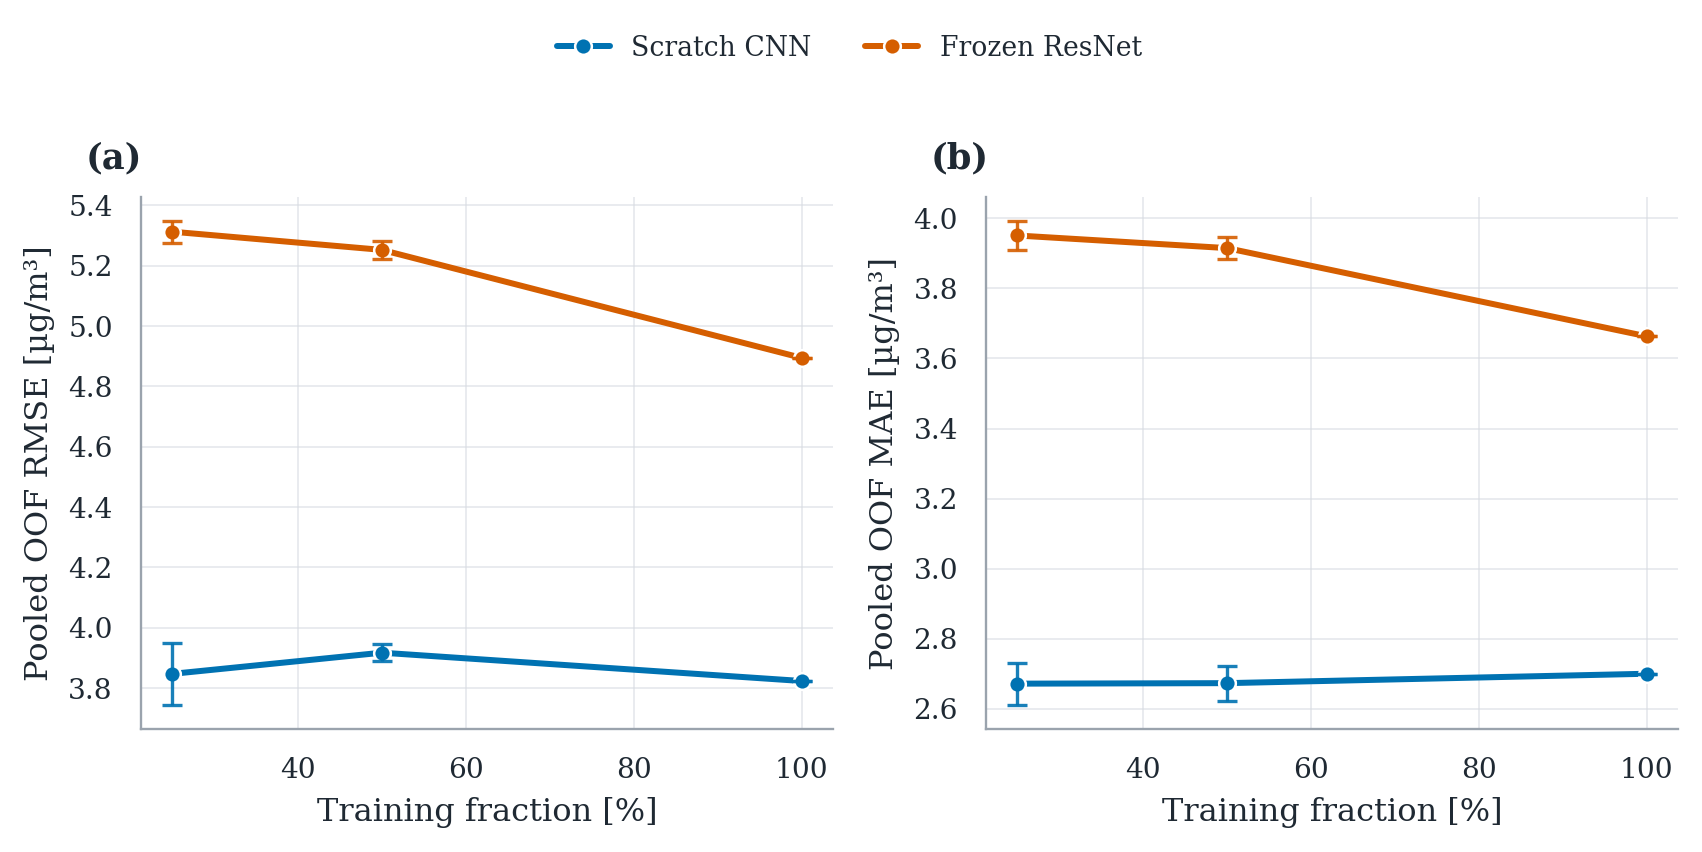
\includegraphics[width=0.72\textwidth]{Figures/generated/data_size_ablation_summary.png}
    \caption{Pooled geographic cross-validation RMSE and MAE for the scratch CNN and frozen ResNet-50 at 25\%, 50\% and 100\% of the development training data.}
    \label{fig:data_size}
\end{figure}


\subsection{Final Training and Sealed TEST Evaluation}
\label{sec:evaluation}

After model selection, \texttt{cnn\_deep\_wide} is trained once on the available development stations after applying a 100 km exclusion buffer around the sealed TEST region. This removes 74 of the 1,869 development stations and leaves 1,795 stations for final training. The model is trained for 24 fixed epochs based on the median best epoch from the original cross-validation used for model selection. No final validation split is used.

Table~\ref{tab:test_summary} reports performance on the 164 sealed TEST stations. The model achieves an RMSE of \SI{2.375}{\micro\gram\per\cubic\meter} and MAE of \SI{1.894}{\micro\gram\per\cubic\meter}. The $R^2$ is strongly negative at $-1.750$. This means that the model explains the within-TEST variation poorly relative to predicting the TEST set's own mean. We treat this as an important sign that spatial generalization remains difficult.

The TEST-set mean is not a deployable baseline because it is only known after observing the held-out labels. Relative to the arithmetic mean of the final training labels, the model reduces RMSE from 2.782 to \SI{2.375}{\micro\gram\per\cubic\meter}. This is an improvement of 14.6\%. Both comparisons are informative. The model beats a training-only constant predictor but still generalizes poorly enough to produce a negative TEST $R^2$.

\begin{table}[ht]
\centering
\caption{Final evaluation of \texttt{cnn\_deep\_wide} on the sealed northern and eastern German TEST region ($n=164$).}
\label{tab:test_summary}
\begin{tabular}{lr}
\toprule
Metric & Value \\
\midrule
MAE & 1.894 \\
RMSE & 2.375 \\
$R^2$ vs.\ TEST mean & -1.750 \\
Bias, prediction $-$ observation & +1.748 \\
Stations overpredicted & 87.2\% \\
Training-mean baseline RMSE & 2.782 \\
RMSE improvement over training-mean baseline & 14.6\% \\
\bottomrule
\end{tabular}
\end{table}

The error also has a clear positive direction. A total of 87.2\% of TEST stations are overpredicted and the mean bias is \SI{1.748}{\micro\gram\per\cubic\meter}. State-level metrics vary considerably but several states contain only a small number of stations. Their individual $R^2$ values are therefore unstable. We use these subgroup results as diagnostics rather than as evidence that the model is generally more reliable in particular urban or rural settings.


\subsection{Implementation of Dense Grid Map}
\label{sec:dense_grid}

We apply the final scratch model to a regular grid with approximately 10 km spacing across the held-out German region. The model produces point predictions at 1,728 usable grid locations. For visualization, the point estimates are connected with a Delaunay triangulation and values are interpolated within each triangle. The continuous-looking surface in Figure~\ref{fig:dense_residual} is therefore a visualization of the model's grid predictions rather than another learned pollution model.

\begin{figure}[ht]
    \centering
    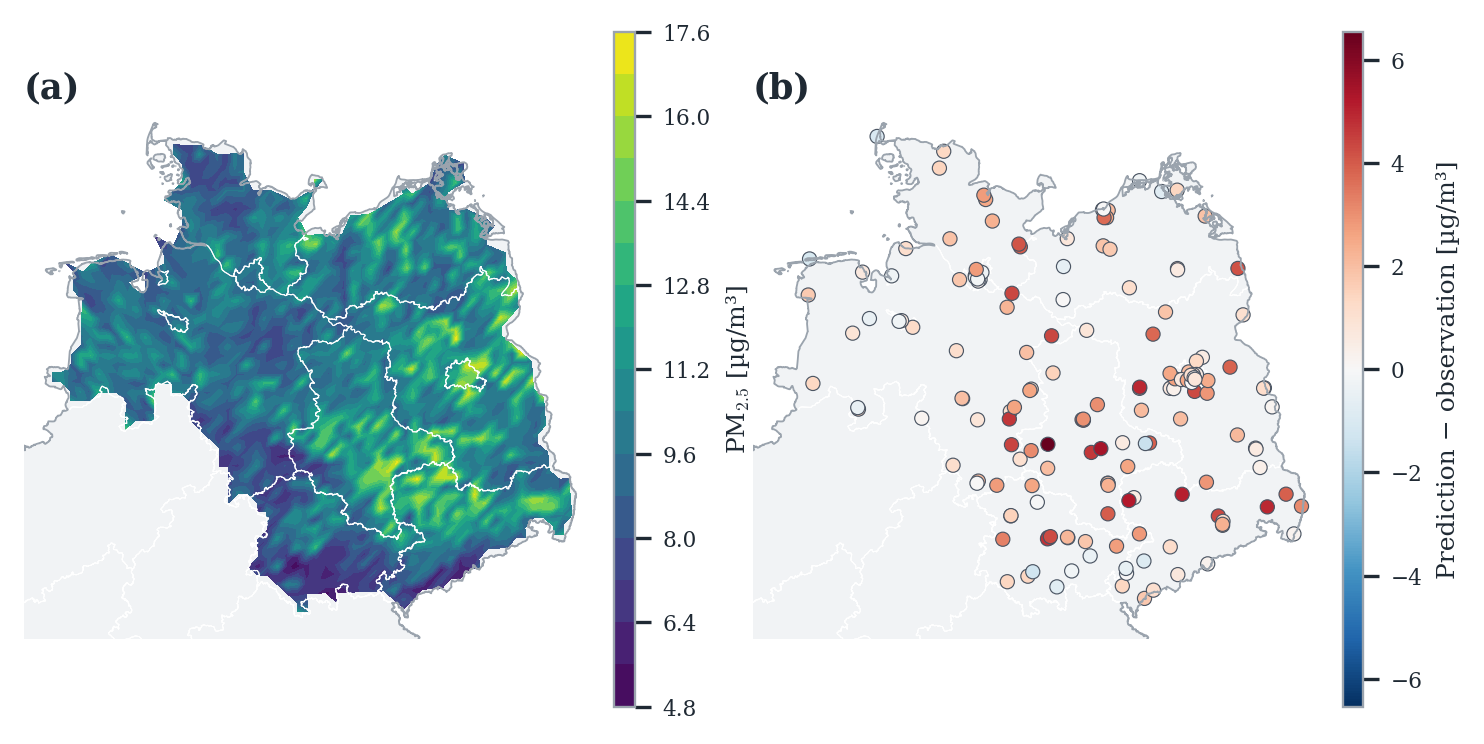
\includegraphics[width=\textwidth]{Figures/generated/dense_prediction_residual_maps.png}
    \caption{Dense PM$_{2.5}$ predictions across the TEST region and residuals at the 164 reference stations. Positive residuals indicate overprediction.}
    \label{fig:dense_residual}
\end{figure}

Across the grid, predicted PM$_{2.5}$ ranges from approximately \SI{5.02}{\micro\gram\per\cubic\meter} to \SI{17.13}{\micro\gram\per\cubic\meter}. Higher predicted values occur in several localized parts of the region including around Berlin and the Leipzig area. These patterns should be interpreted descriptively. The sealed TEST evaluation shows systematic overprediction and heterogeneous errors, so the dense surface should not be treated as a substitute for monitoring observations or as direct evidence of intervention priorities.


\section{Socio-Economic Analysis}
\label{sec:socioeconomic}

\subsection{Aggregation of Predicted PM$_{2.5}$ to Kreis Level}
\label{sec:kreis_aggregation}

The dense predictions are produced on a regular grid rather than directly for administrative units. To combine them with the socioeconomic data, each grid point is assigned to the Kreis polygon containing its center coordinates. Predicted PM$_{2.5}$ is then averaged across all grid points within each Kreis.

Of the 1,728 usable grid predictions, 1,719 are assigned to a Kreis. This produces modeled pollution estimates for 134 Kreise within the prediction domain. The number of contributing grid points ranges from 1 to 54 with a median of 12.

Our main pollution measure is therefore the arithmetic mean of the modeled PM$_{2.5}$ values across grid points inside each Kreis. It should be interpreted as an area-oriented estimate of mean modeled ambient pollution rather than as population-weighted individual exposure. Constructing a population-weighted measure would require information on the within-Kreis spatial distribution of the population.

Across the 134 covered Kreise, mean predicted PM$_{2.5}$ ranges from approximately \SI{6.02}{\micro\gram\per\cubic\meter} to \SI{13.12}{\micro\gram\per\cubic\meter} with an overall Kreis mean of \SI{9.88}{\micro\gram\per\cubic\meter}.


\subsection{Spatial Patterns}
\label{sec:socio_patterns}

The modeled PM$_{2.5}$ surface and socioeconomic variables vary spatially across the study region. The full set of descriptive socioeconomic maps is kept in the appendix because the main report is limited to ten pages. The maps do not indicate one simple socioeconomic gradient. We therefore compare mean modeled PM$_{2.5}$ with the selected Kreis-level indicators quantitatively.


\subsection{Association with Socioeconomic Characteristics}
\label{sec:socio_assoc}

Table~\ref{tab:socio_correlations} reports descriptive Pearson correlations. The associations are generally weak. The strongest positive association is with unemployment at $r=0.225$. University-degree share follows at $r=0.198$ and log population density at $r=0.171$. Disposable income is weakly negatively associated with modeled PM$_{2.5}$ at $r=-0.145$ while immigration history shows essentially no linear association at $r=-0.022$.

\begin{table}[ht]
\centering
\caption{Pearson correlations between Kreis-level mean modeled PM$_{2.5}$ and selected socioeconomic and demographic indicators.}
\label{tab:socio_correlations}
\begin{tabular}{lrr}
\toprule
Indicator & $n$ & Pearson $r$ \\
\midrule
Disposable income per capita & 132 & -0.145 \\
Unemployment rate & 134 & 0.225 \\
No vocational qualification & 134 & -0.153 \\
University degree & 134 & 0.198 \\
Immigration history & 134 & -0.022 \\
Log population density & 134 & 0.171 \\
Population aged 65+ & 134 & -0.120 \\
\bottomrule
\end{tabular}
\end{table}

Overall, these results provide little evidence for a strong or uniform socioeconomic gradient in modeled PM$_{2.5}$ across the covered Kreise. Some indicators point weakly in a disadvantage direction such as lower income and higher unemployment. Other indicators do not follow the same direction. The share without a vocational qualification is weakly negative, university-degree share is weakly positive and immigration history is close to zero. The pattern therefore cannot be summarized by a single dimension of socioeconomic disadvantage.

The analysis also inherits the limitations of the pollution model. The Kreis-level values are predictions rather than direct measurements, the TEST evaluation shows systematic bias and the exposure measure is not population-weighted. The results should therefore be read as exploratory spatial associations rather than as evidence of causal environmental inequality or individual exposure differences.


\section{Conclusion}
\label{sec:conclusion}

This project develops a multimodal remote-sensing pipeline for annual PM$_{2.5}$ prediction under geographic holdout. We first investigated whether Sensor.Community measurements could increase the number of available labels. The raw annual measurements show very large errors. Annual percentile mapping and regression corrections reduce some of this error but they do not produce a reliable combination of low error and preserved spatial variation. The HYRAS experiment shows that humidity and temperature explain part of the daily sensor error. This daily improvement does not translate into sufficiently reliable annual labels. We therefore use official EEA measurements as the only labels for the final deep-learning models.

The main model comparison shows a clear advantage for the scratch CNN over the evaluated BigEarthNet-pretrained ResNet-50 configurations. We tested both a frozen backbone and a fully trainable diagnostic variant. Unfreezing the pretrained backbone did not produce a noticeable improvement on the diagnostic fold. The data-size ablation leads to the same broader conclusion because the pretrained model remains worse when fewer labeled stations are available.

On the sealed northern and eastern German TEST region, the selected scratch model improves RMSE by 14.6\% over a deployable training-mean baseline. At the same time, the strongly negative $R^2$, positive bias and high fraction of overpredicted stations show that spatial generalization remains limited. The dense grid demonstrates how the model can produce estimates away from monitoring stations but the resulting surface should be treated as model-based rather than measured pollution.

Finally, the Kreis-level analysis finds only weak and inconsistent associations between modeled PM$_{2.5}$ and the selected socioeconomic indicators. This does not support a strong single environmental-inequality gradient in the covered region. A stronger exposure analysis would require more reliable pollution predictions and population-weighted exposure measures.

The project has several limitations. Annual averaging removes short-term pollution dynamics. The final prediction model does not include detailed meteorological variables beyond the satellite-derived atmospheric context. The official reference network remains spatially uneven and the low-cost network could not be used as reliable annual labels. The 100 km buffer reduces spatial dependence but it does not remove every possible overlap introduced by the widest contextual inputs. Future work could add meteorological covariates, quantify predictive uncertainty, test other pretrained remote-sensing backbones and evaluate population-weighted exposure once sufficiently detailed population data are available.


\bibliography{references}


\appendix
\section{Additional Graphs and Images}

\subsection{Generic Sentinel-2 Patch Examples}

% TODO: replace in the main report with reproducibly selected high/low-PM2.5 examples
% once the JupyterHub patch arrays are available.
\begin{figure}[H]
    \centering
    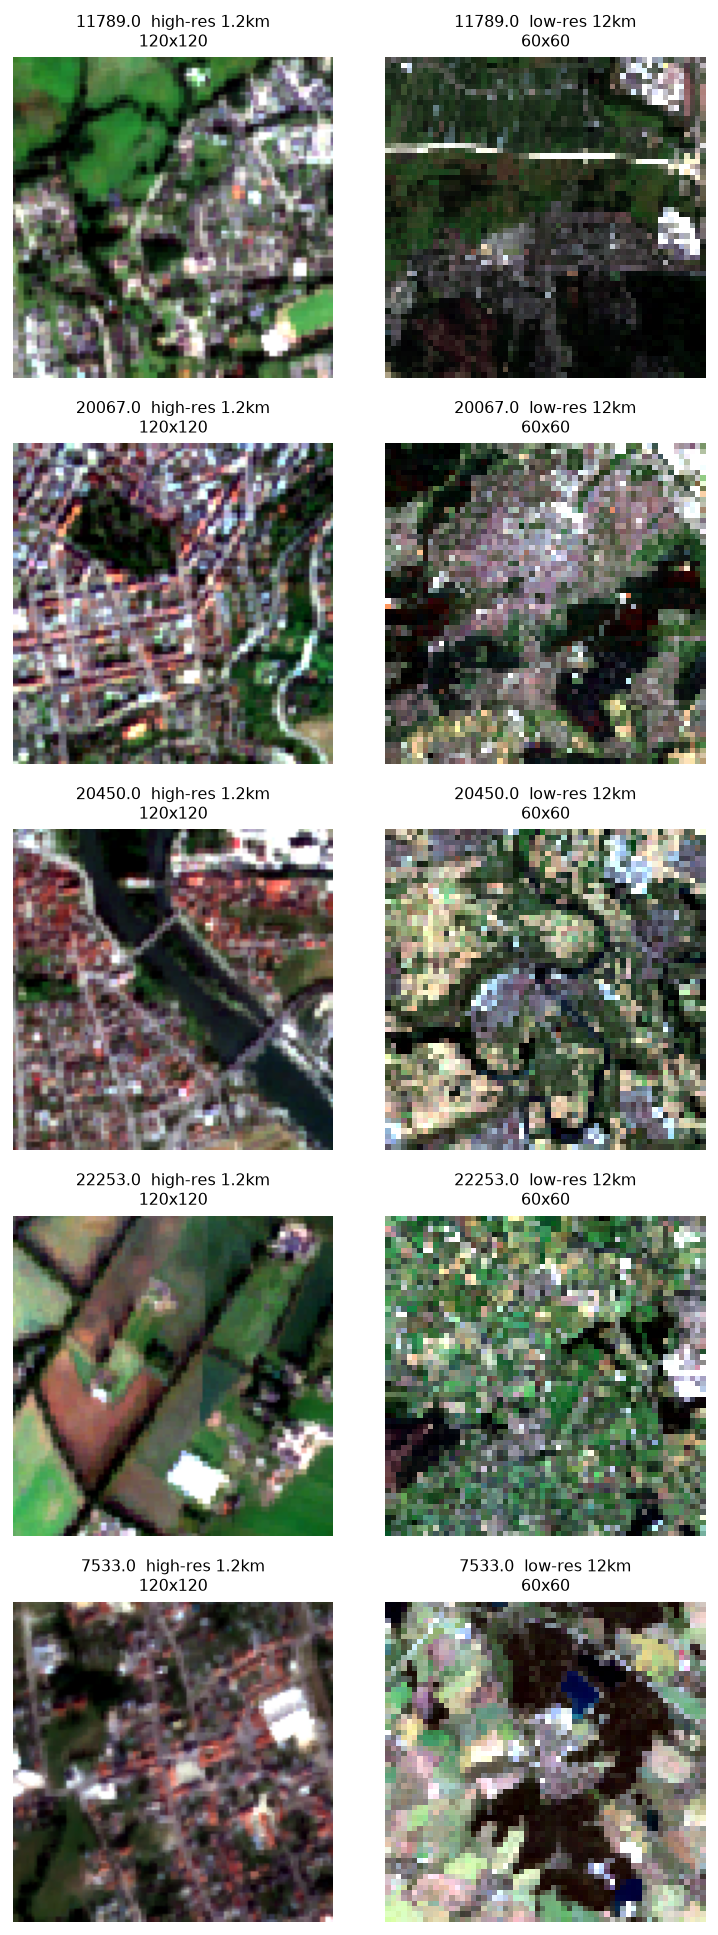
\includegraphics[width=0.55\textwidth]{Figures/generated/preview_patches.png}
    \caption{Examples of the currently available high-resolution and low-resolution Sentinel-2 patch visualization.}
    \label{fig:patch_preview}
\end{figure}


\subsection{Objective-Loss Learning Curves}

\begin{figure}[H]
    \centering
    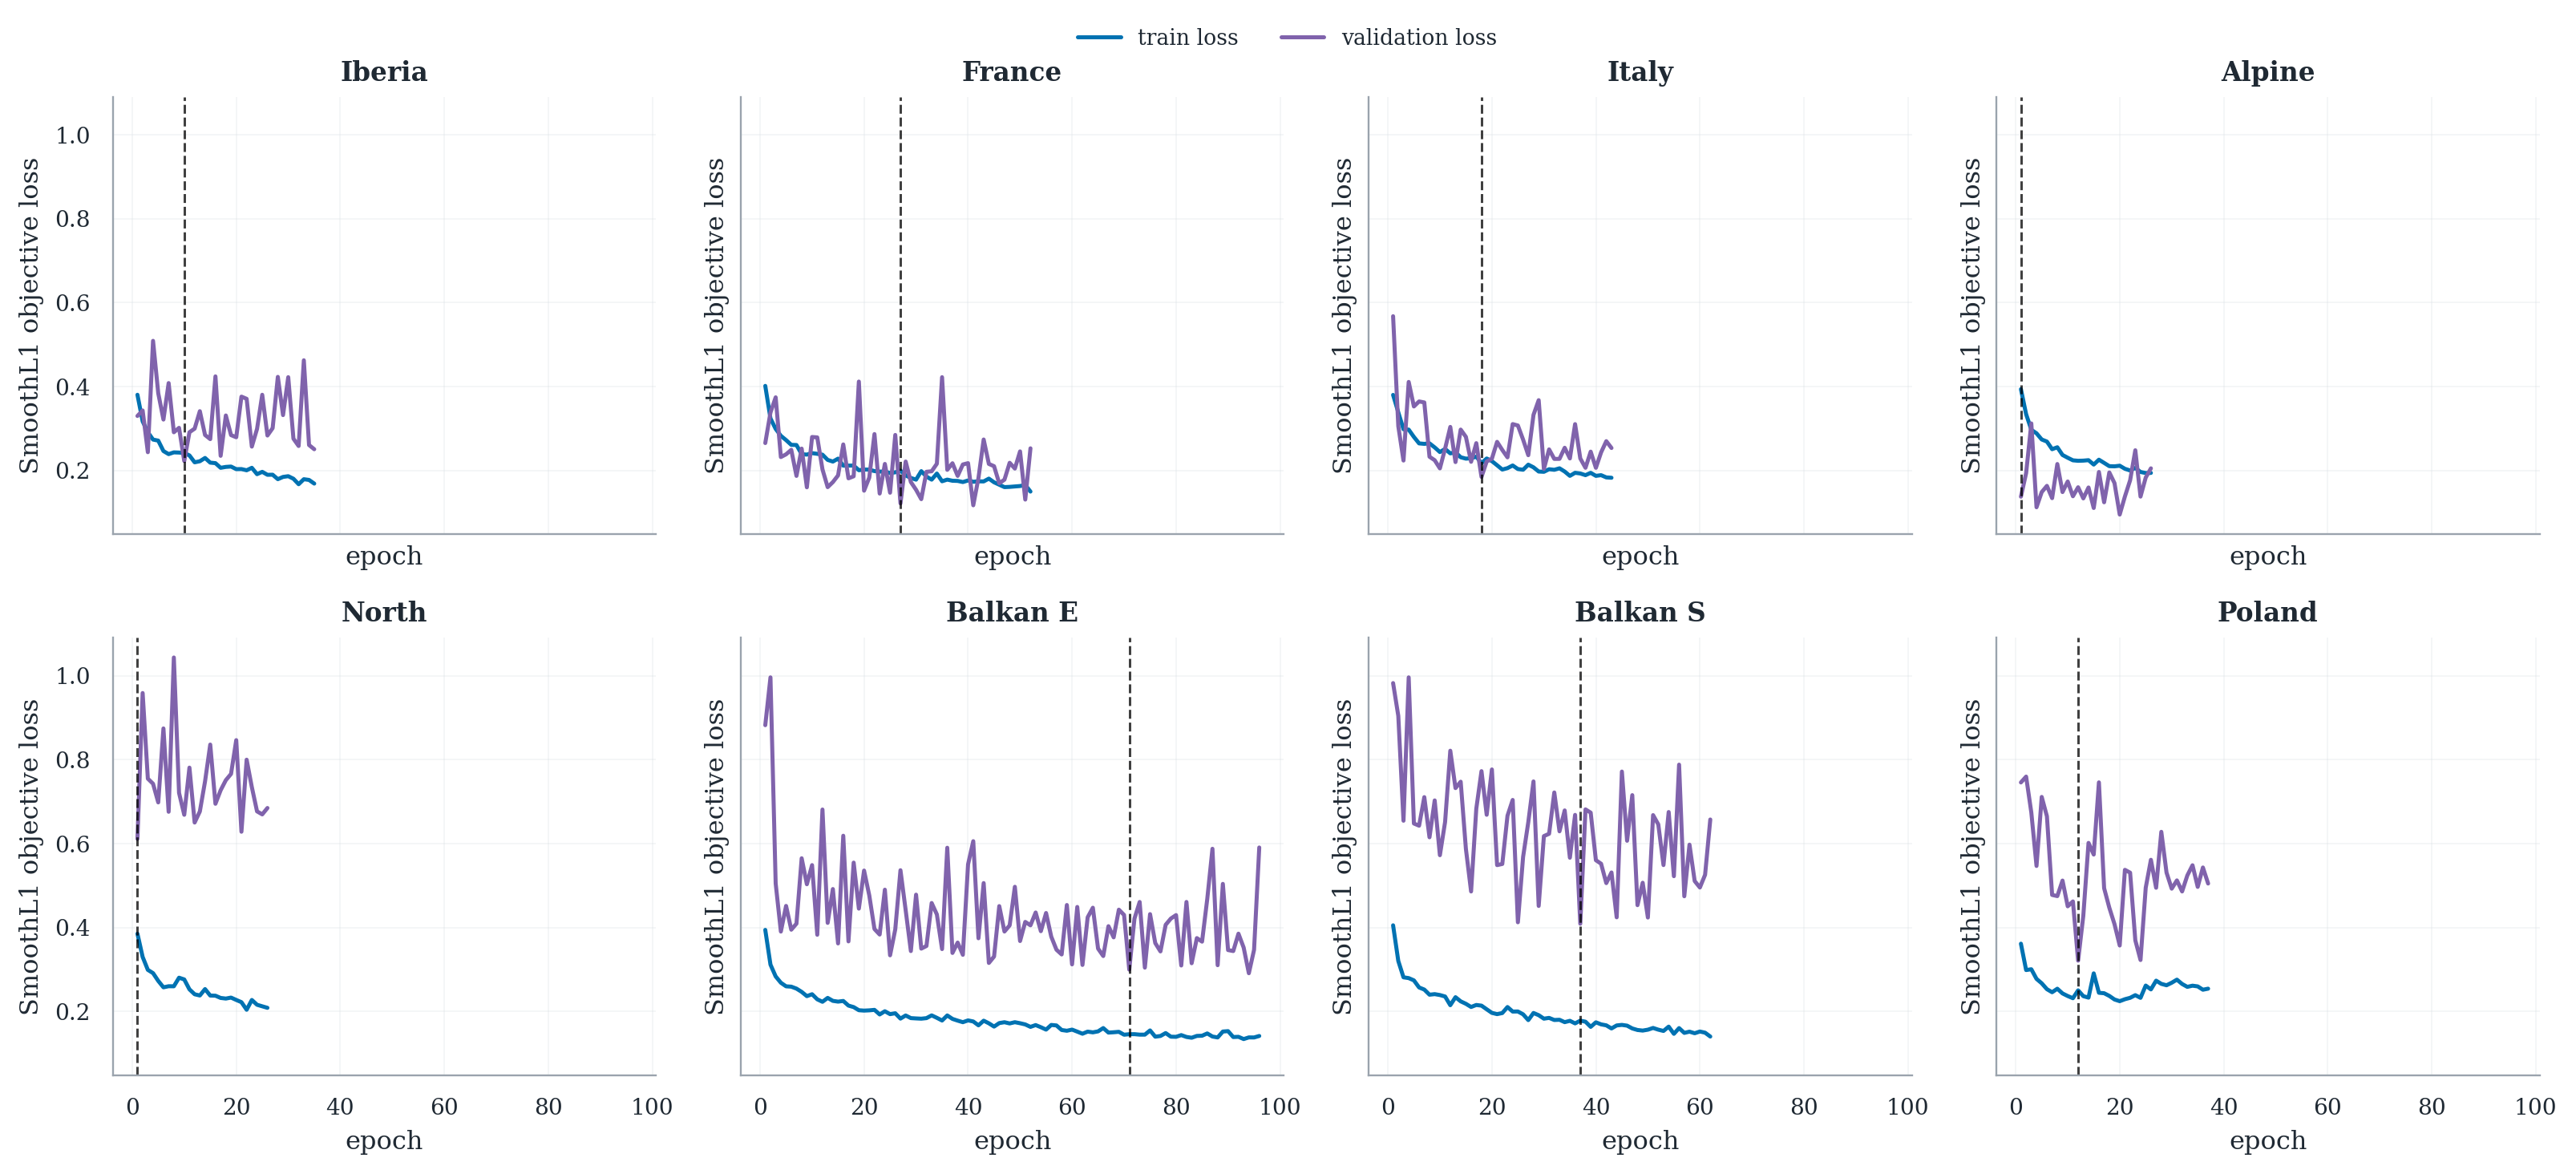
\includegraphics[width=\textwidth]{Figures/generated/learning_curves_cnn_deep_wide_objective_loss.png}
    \caption{SmoothL1 objective-loss curves across the eight geographic folds for the scratch CNN.}
    \label{fig:scratch_loss}
\end{figure}

\begin{figure}[H]
    \centering
    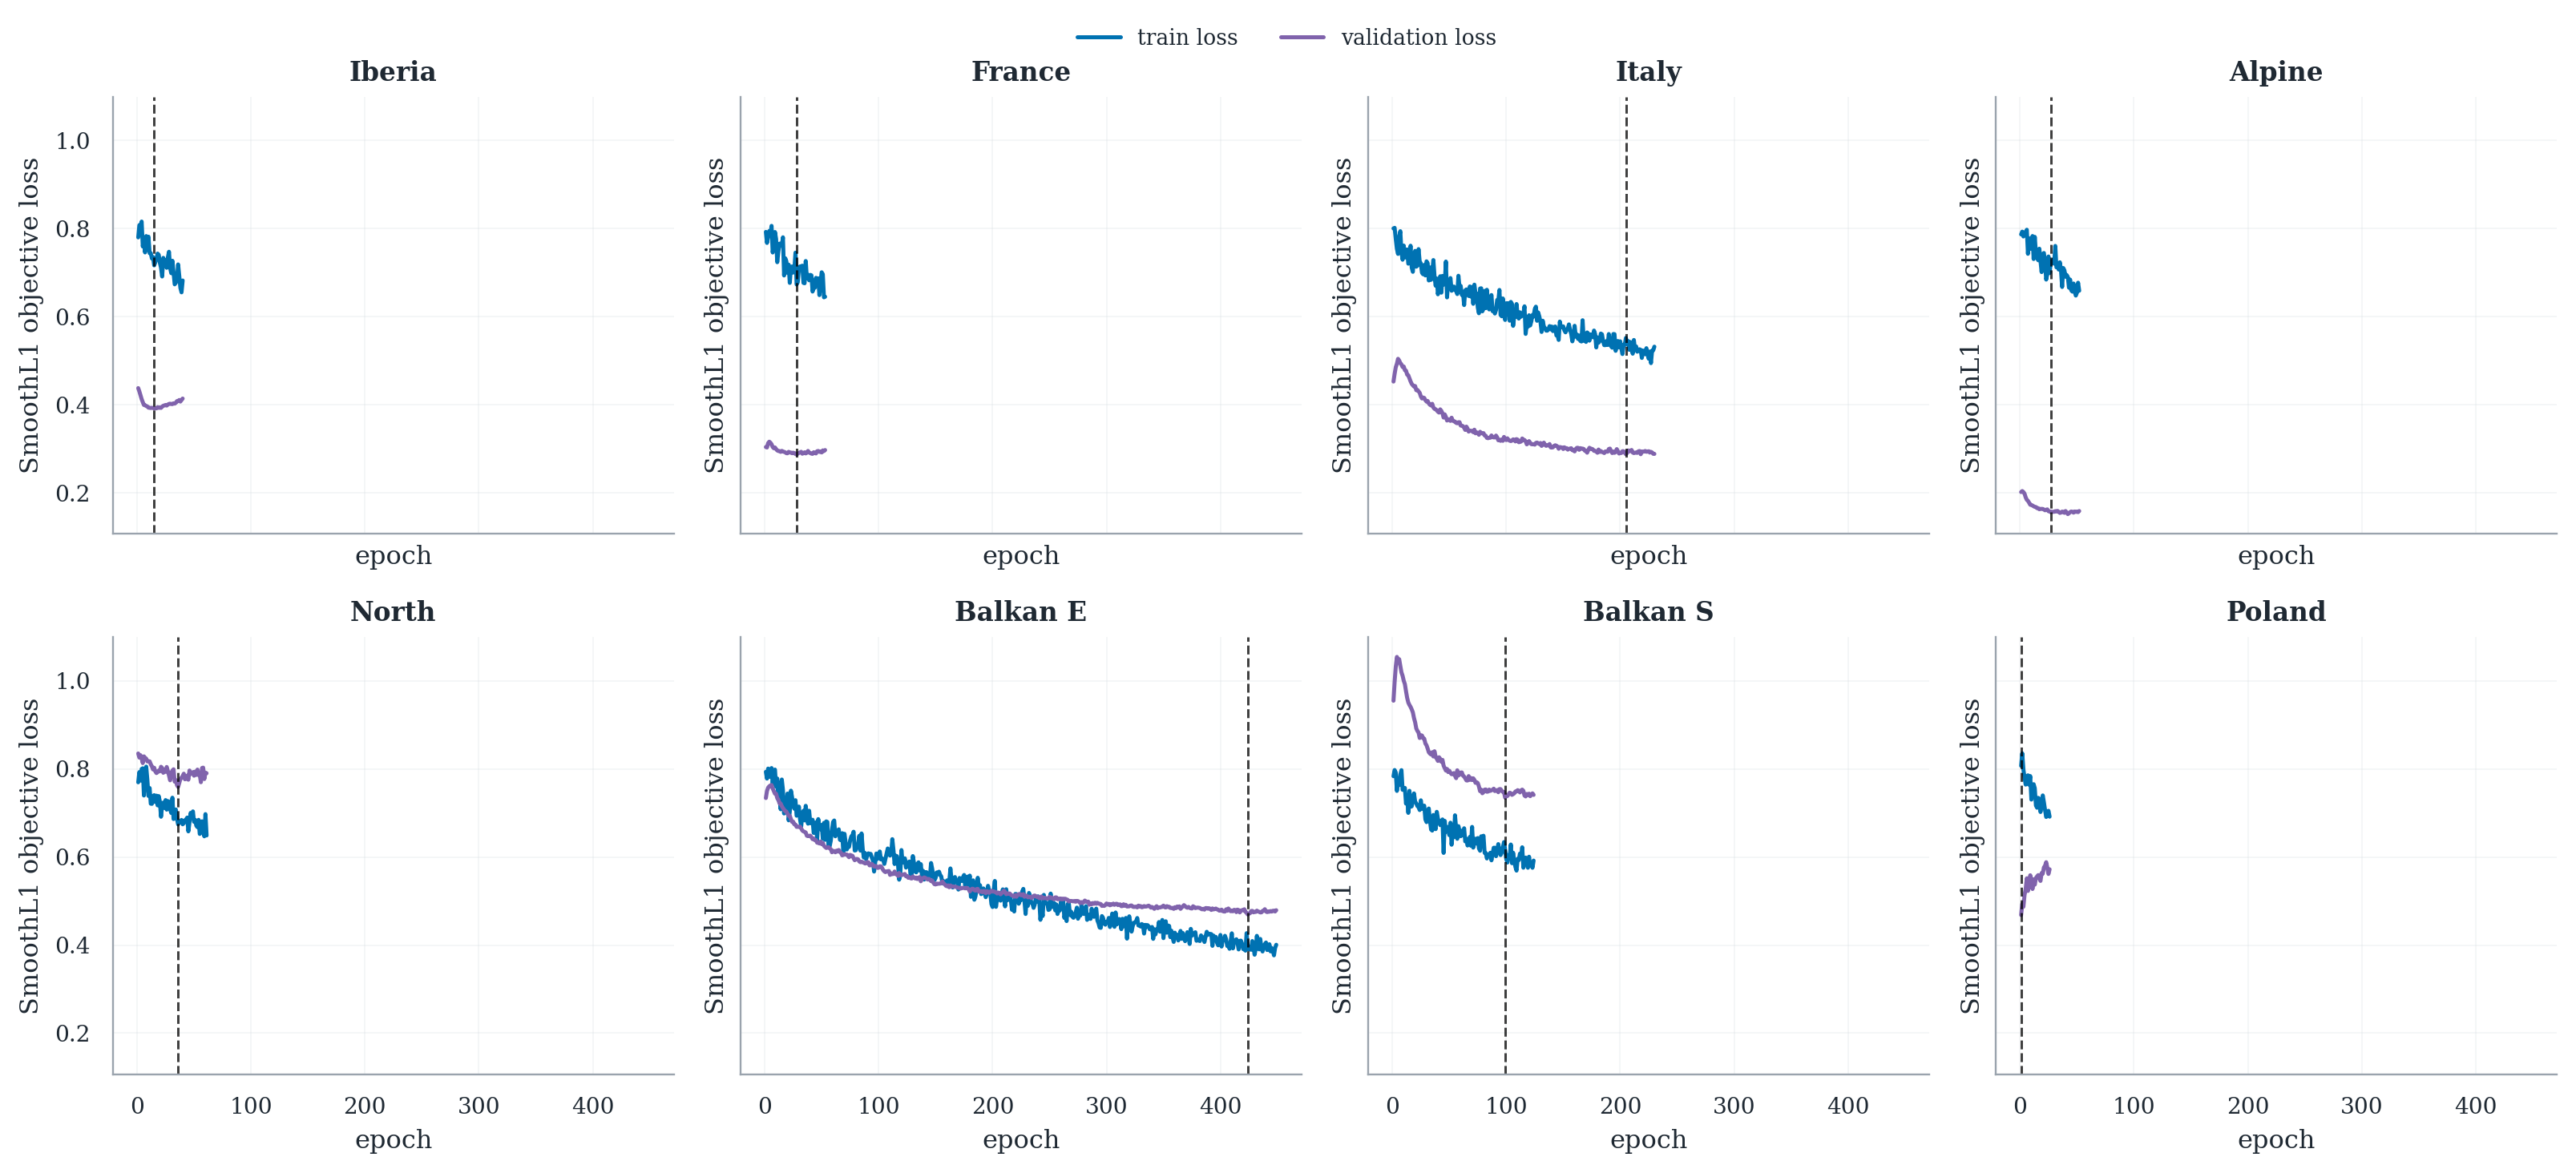
\includegraphics[width=\textwidth]{Figures/generated/learning_curves_resnet_frozen_objective_loss.png}
    \caption{SmoothL1 objective-loss curves across the eight geographic folds for the frozen-backbone ResNet-50.}
    \label{fig:resnet_loss}
\end{figure}


\subsection{Socio-Economic Diagnostics}

\begin{figure}[H]
    \centering
    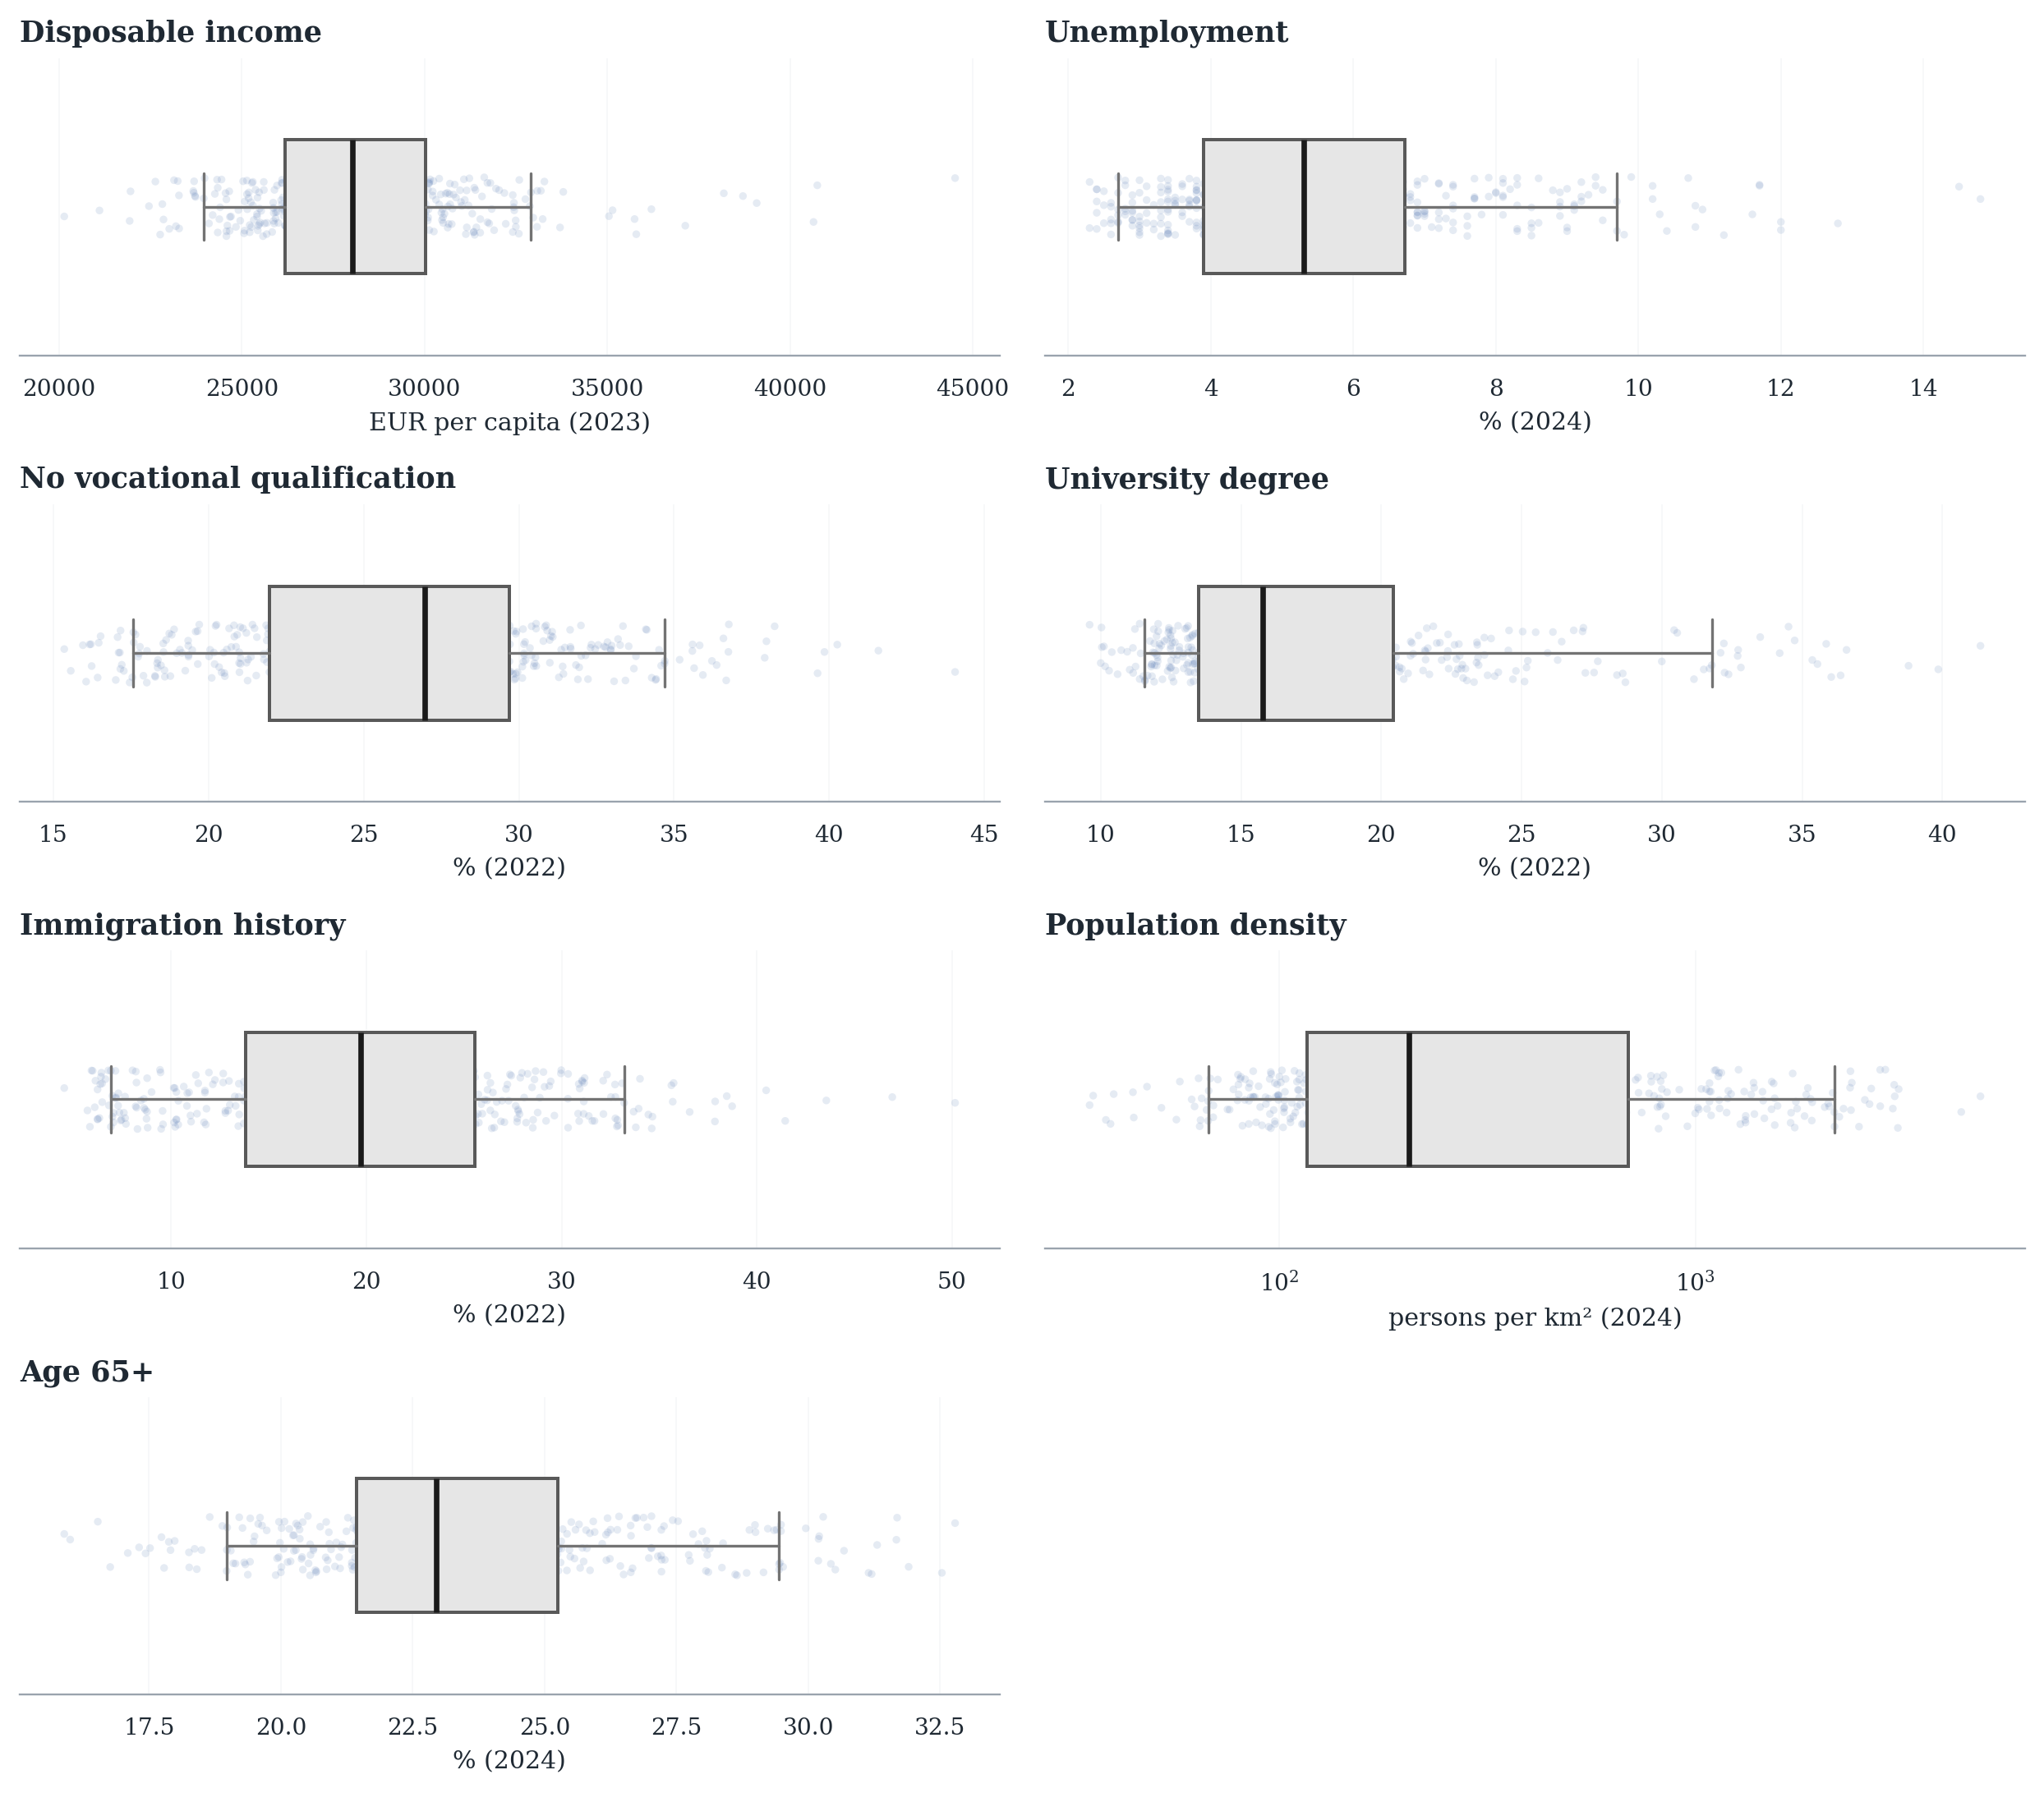
\includegraphics[width=0.75\textwidth]{Figures/generated/socioeconomic_indicator_boxplots.png}
    \caption{Distributions of selected socioeconomic and demographic indicators across German Kreise.}
    \label{fig:socio_boxplots}
\end{figure}

\begin{figure}[H]
    \centering
    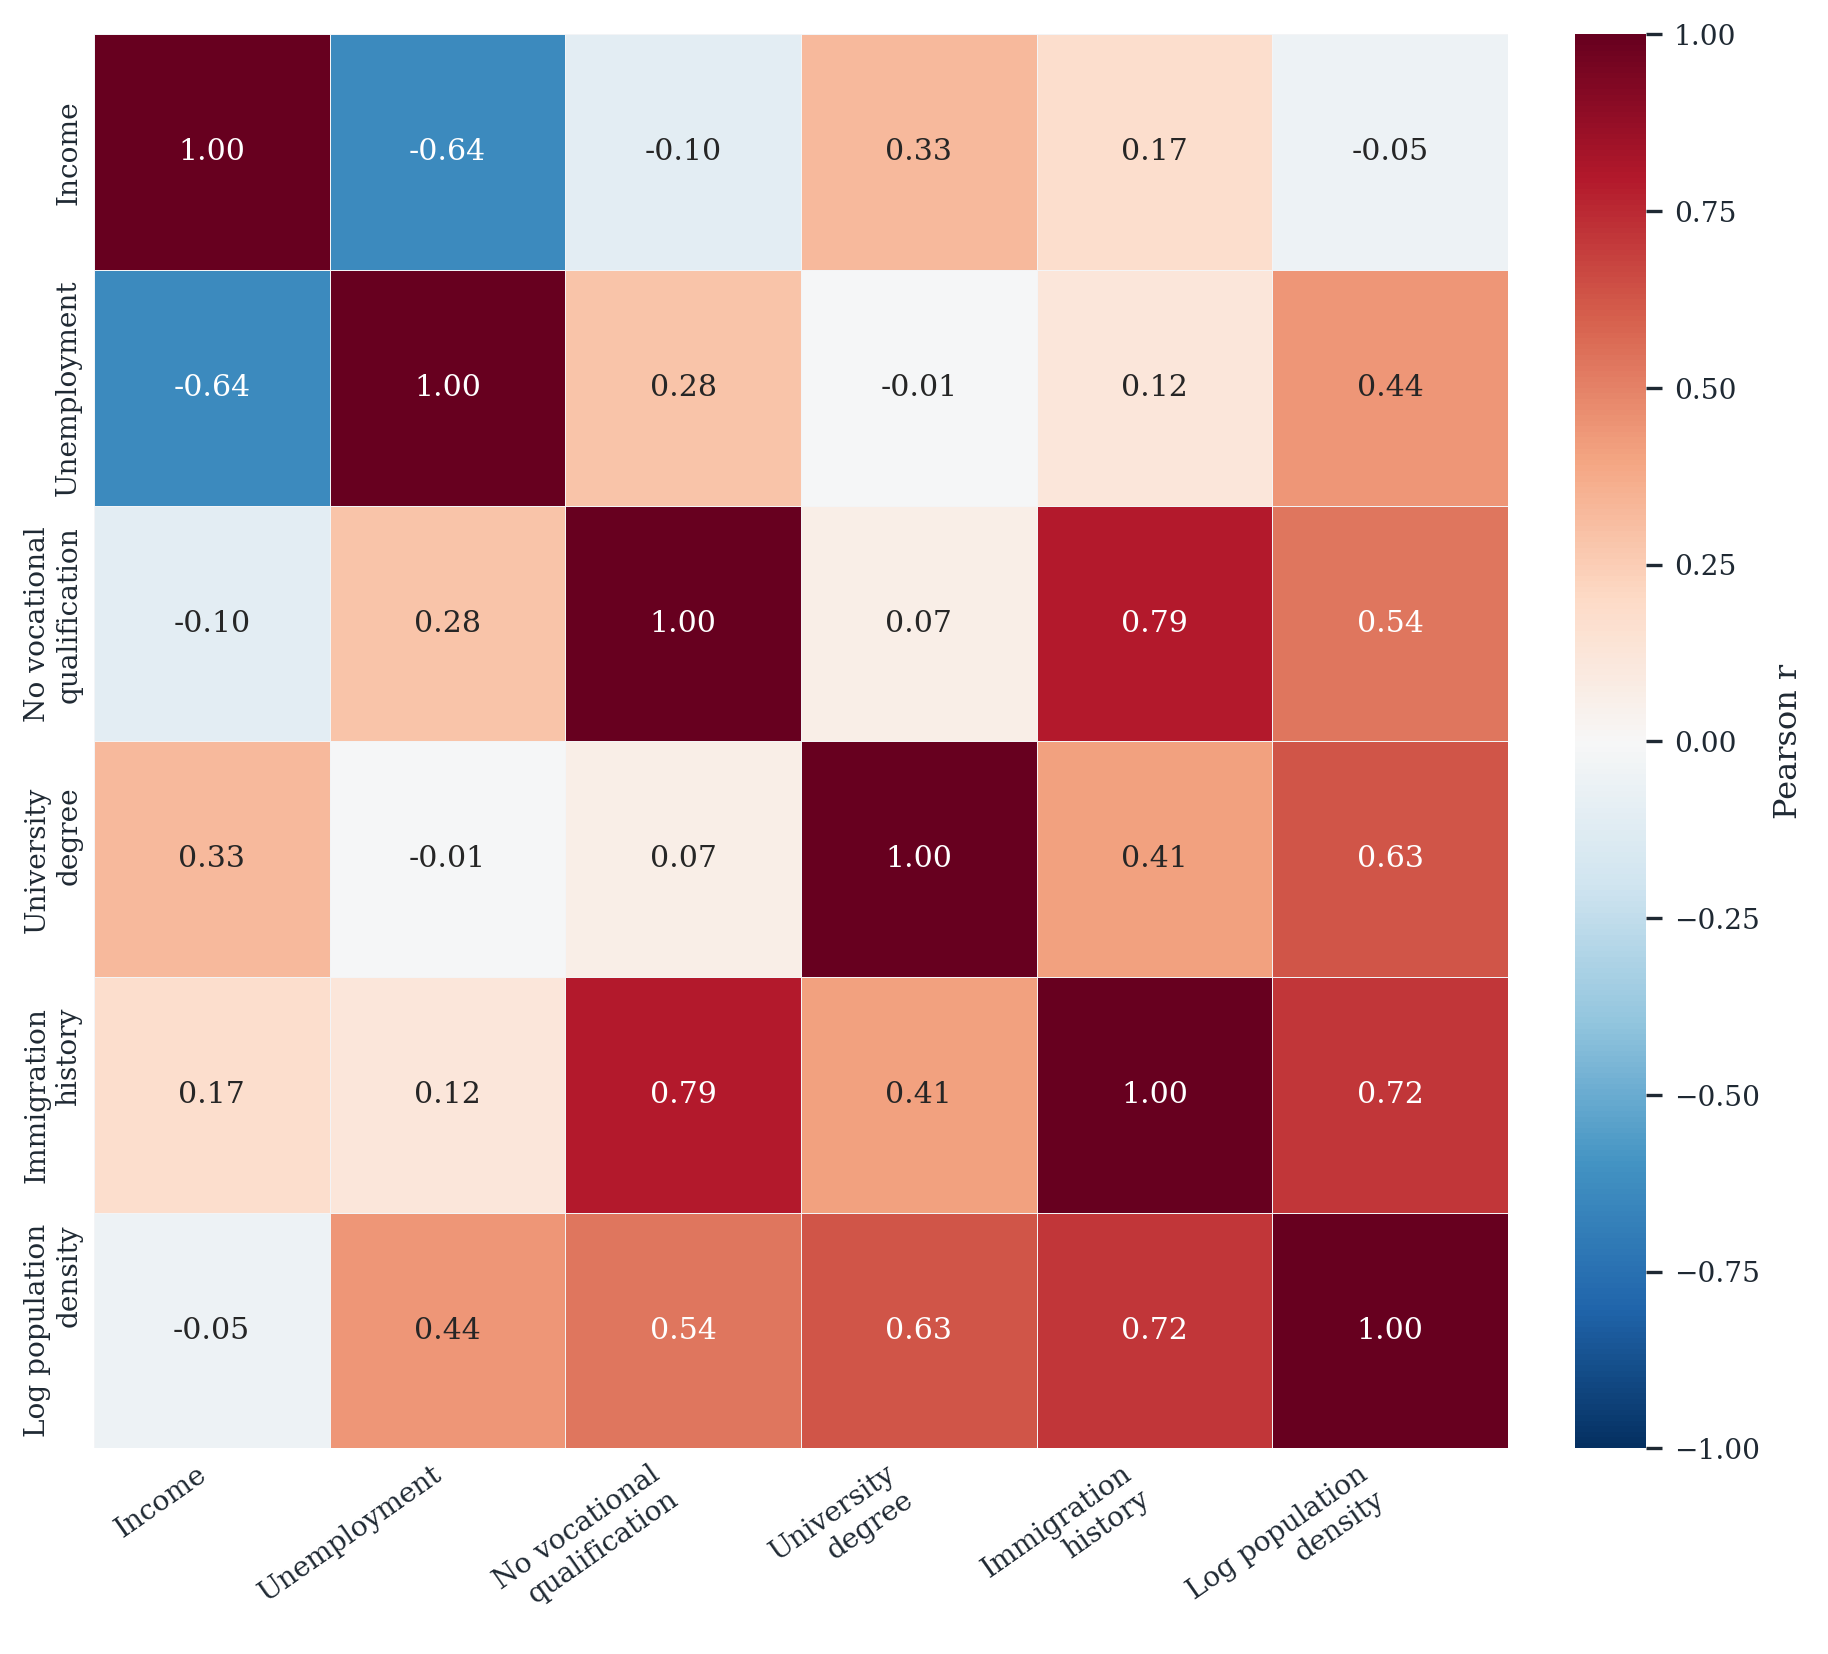
\includegraphics[width=0.65\textwidth]{Figures/generated/socioeconomic_correlation_matrix.png}
    \caption{Pearson correlations among selected socioeconomic indicators across German Kreise.}
    \label{fig:socio_matrix}
\end{figure}

\begin{figure}[H]
    \centering
    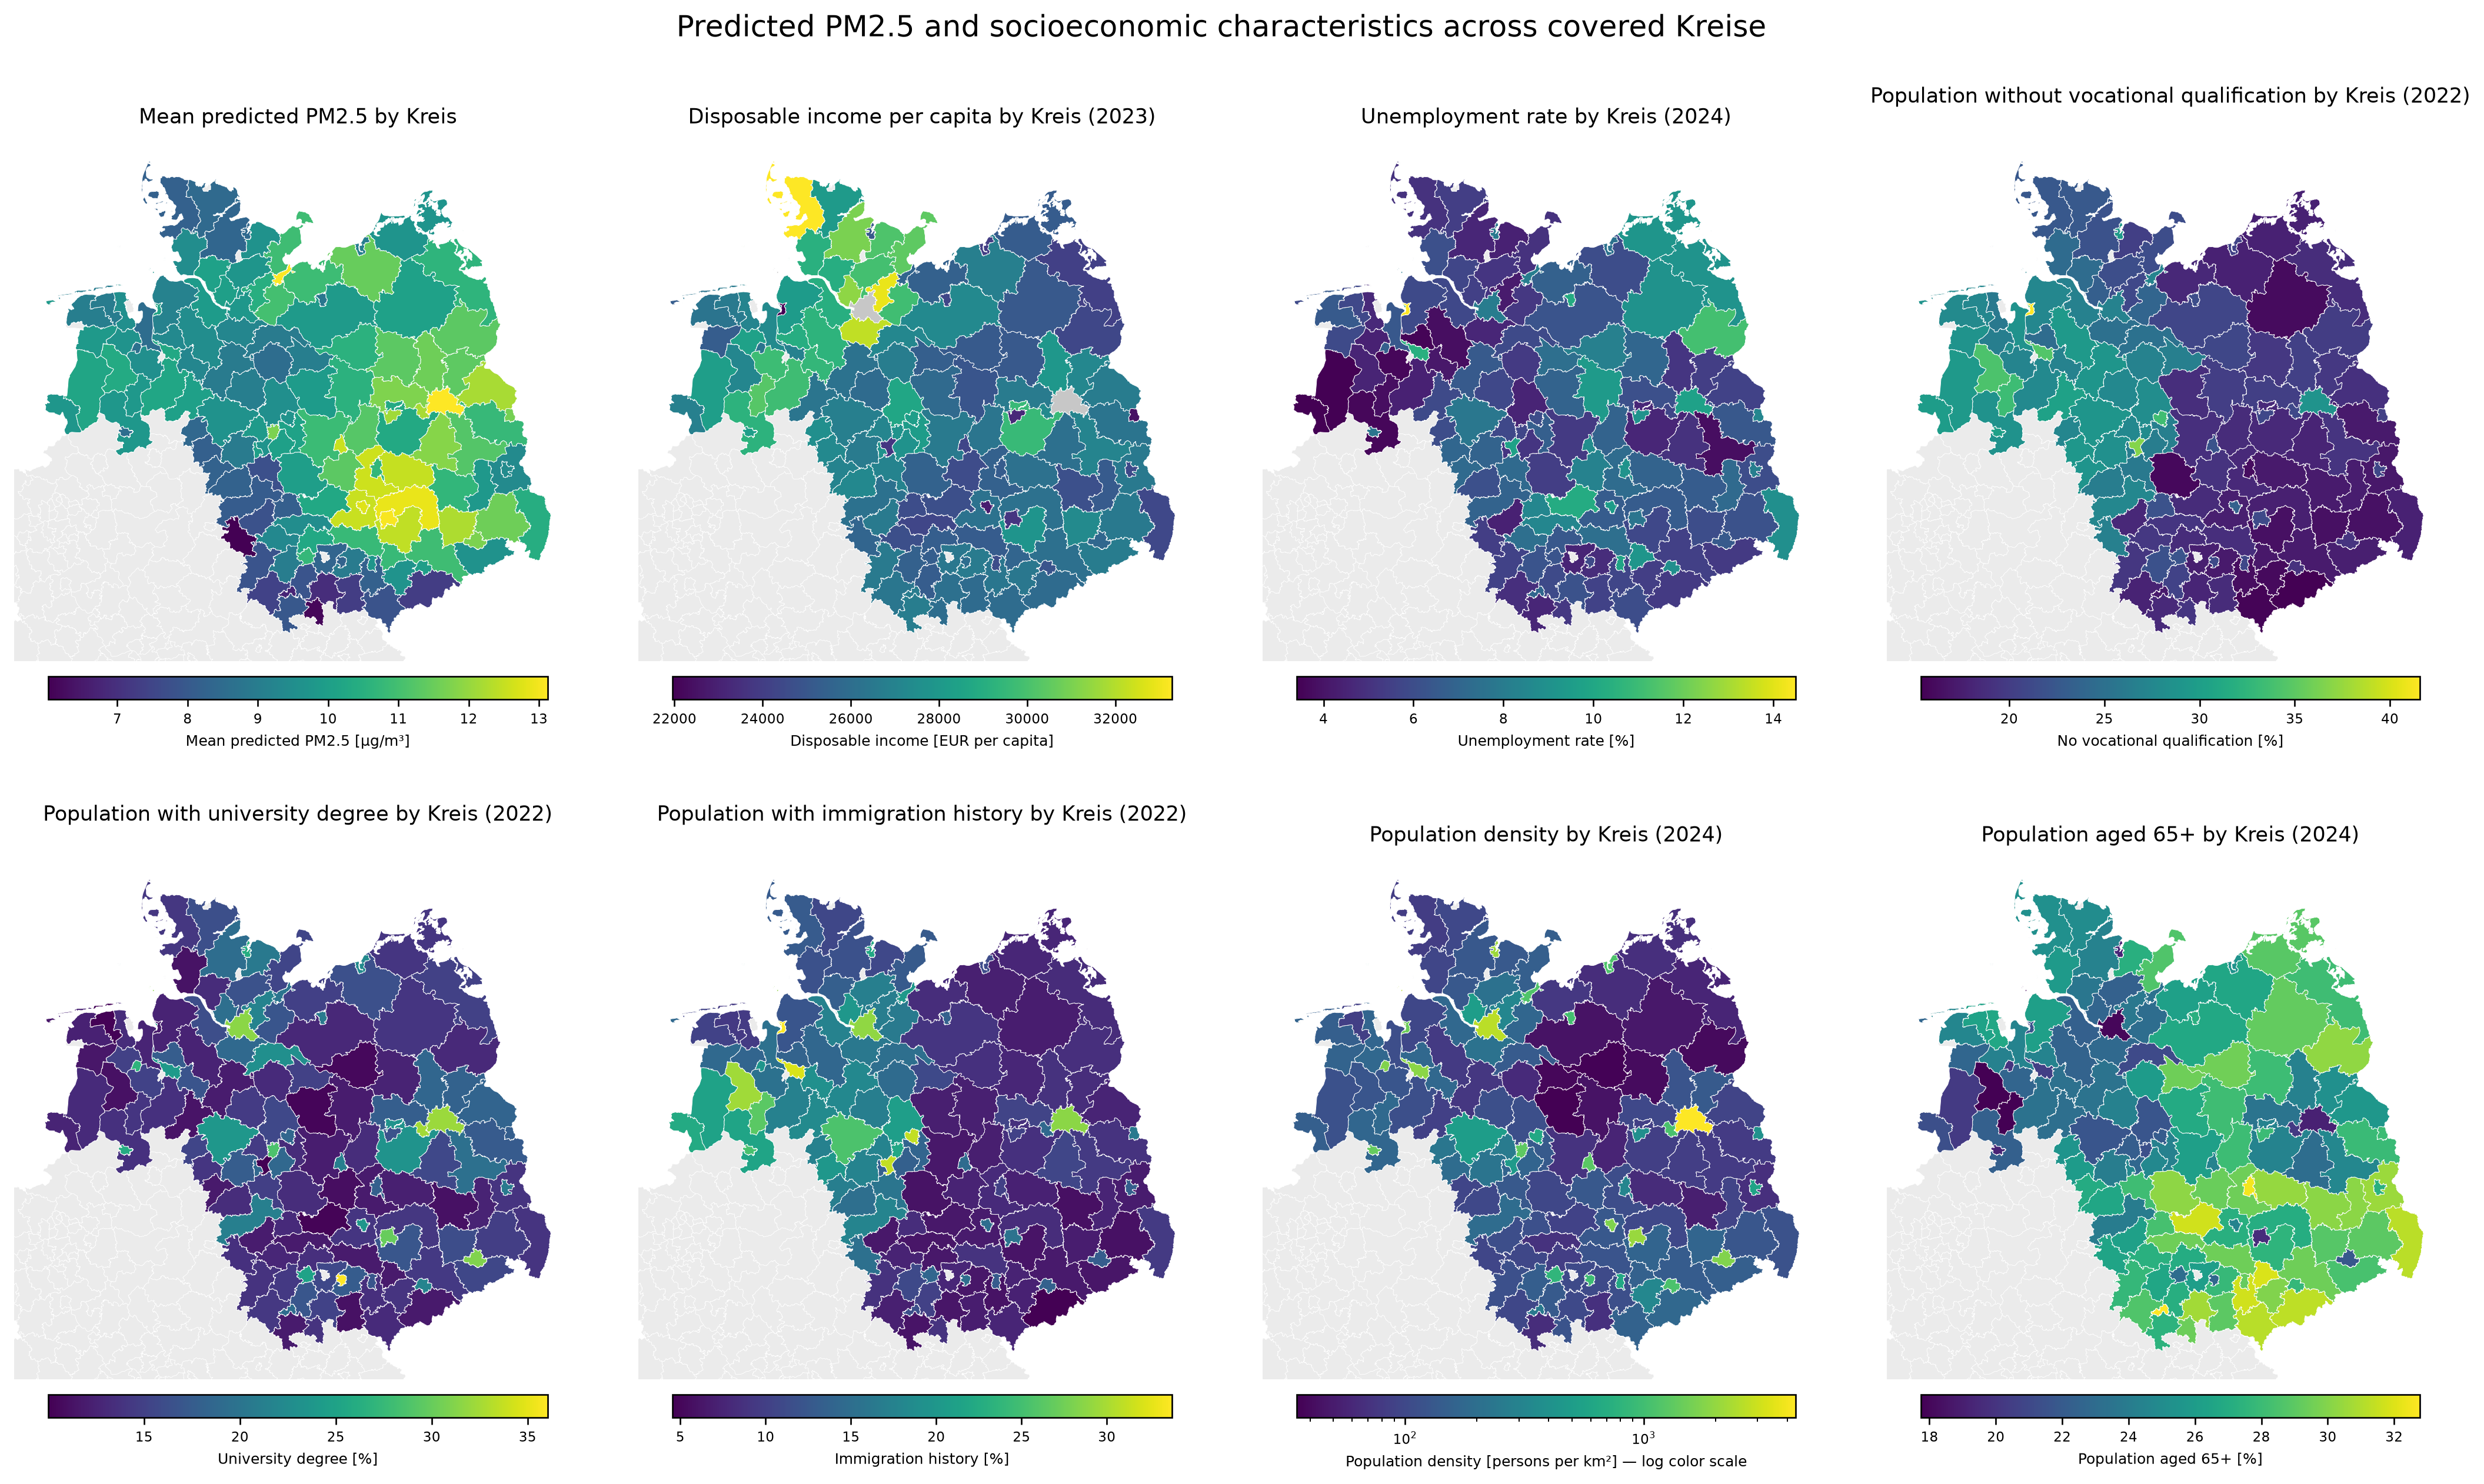
\includegraphics[width=\textwidth]{Figures/generated/socioeconomic_summary_maps.png}
    \caption{Spatial distribution of modeled PM$_{2.5}$ and selected socioeconomic and demographic indicators across the covered Kreise. Population density is displayed on a logarithmic scale.}
    \label{fig:socio_maps}
\end{figure}


\subsection{State-Level TEST Diagnostics}

\begin{table}[H]
\centering
\small
\caption{TEST-set diagnostics by German federal state. State-level $R^2$ values should be interpreted cautiously because several states have small samples and narrow outcome ranges.}
\label{tab:test_state}
\begin{tabular}{lrrrr}
\toprule
State & $n$ & Bias & MAE & $R^2$ \\
\midrule
Berlin & 12 & 1.182 & 1.182 & 0.235 \\
Hamburg & 8 & 0.394 & 0.678 & -2.384 \\
Bremen & 4 & 0.370 & 0.625 & -26.02 \\
Sachsen & 19 & 2.052 & 2.146 & -1.790 \\
Niedersachsen & 29 & 1.574 & 1.712 & -4.410 \\
Mecklenburg-Vorpommern & 18 & 1.313 & 1.495 & -6.931 \\
Thueringen & 21 & 1.738 & 2.054 & -4.744 \\
Brandenburg & 25 & 1.853 & 1.853 & -7.683 \\
Schleswig-Holstein & 10 & 2.381 & 2.579 & -8.270 \\
Sachsen-Anhalt & 18 & 2.944 & 3.105 & -7.038 \\
\bottomrule
\end{tabular}
\end{table}


\end{document}
